\tdplotsetmaincoords{60}{120}
\begin{tikzpicture}
	[scale=6,
		tdplot_main_coords,
		axis/.style={->,black,thick},
		vector/.style={-stealth,black, thick},
		vector guide/.style={dashed,black,thick},
		angle/.style={black,thick}]

	%standard tikz coordinate definition using x, y, z coords
	\coordinate (O) at (0,0,0);
	
	%tikz-3dplot coordinate definition using r, theta, phi coords
	\tdplotsetcoord{P}{.8}{55}{60}
	
	%draw axes
	\draw[axis] (0,0,0) -- (1,0,0) node[anchor=north east]{$x$};
	\draw[axis] (0,0,0) -- (0,1,0) node[anchor=north west]{$y$};
	\draw[axis] (0,0,0) -- (0,0,1) node[anchor=south]{$z$};
	
	%draw a vector from O to P
	\draw[vector] (O) -- (P);
	
	%draw guide lines to components
	\draw[vector guide] (O) -- (Pxy);
	\draw[vector guide] (Pxy) -- (P);
	
	%draw an arc illustrating the angle defining the orientation
	\tdplotdrawarc[angle]{(O)}{.35}{0}{60}{anchor=north}{$\phi$}

	%define the rotated coordinate frame to lie in the "theta plane"
	\tdplotsetthetaplanecoords{55}
	
	\tdplotdrawarc[tdplot_rotated_coords,angle]{(O)}{.35}{0}{55}
          {anchor=south west}{$\theta$}

\end{tikzpicture}
%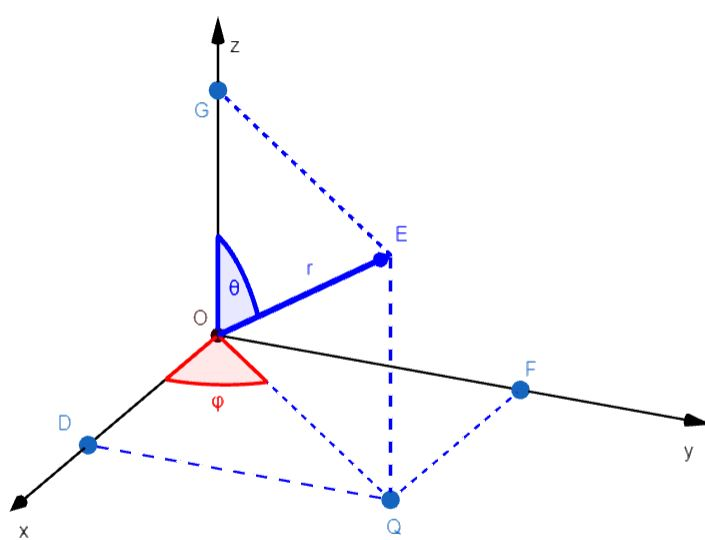
\includegraphics[scale=.6]{spherical.jpg}

